\documentclass[10pt,a4paper]{article}

\usepackage[T1]{fontenc}
\usepackage[utf8]{inputenc}
\usepackage{lmodern}
\usepackage[margin=18mm,top=17mm,bottom=19mm]{geometry}
\usepackage{microtype}
\usepackage{amsmath,amssymb}
\usepackage{booktabs}
\usepackage{graphicx}
\usepackage{caption}
\usepackage{float}
\usepackage{enumitem}
\usepackage{siunitx}
\usepackage{xcolor}
\usepackage{xurl}
\usepackage{listings}
\usepackage{fancyhdr}
\usepackage{lastpage}
\usepackage{cite}
\usepackage[
  colorlinks=true,
  linkcolor=blue!55!black,
  citecolor=blue!55!black,
  urlcolor=blue!55!black,
  pdfauthor={Timofei Amosov},
  pdftitle={FractalFlow: Portable Deep-Zoom Julia Rendering with Perturbation Theory across WebGPU and CUDA},
  pdfsubject={Technical report, version 1.1.0},
  pdfkeywords={Julia set, deep zoom, perturbation theory, WebGPU, CUDA, double-double arithmetic}
]{hyperref}

\graphicspath{{figures/}}
\setlist{nosep,leftmargin=1.4em}
\captionsetup{font=small,labelfont=bf}
\sisetup{detect-all,group-separator={,},group-minimum-digits=4}
\setlength{\parindent}{1em}
\setlength{\parskip}{0.15em}
\setcounter{secnumdepth}{2}

\definecolor{codebg}{HTML}{F4F6F8}
\definecolor{codeframe}{HTML}{D0D5DD}
\lstset{
  basicstyle=\ttfamily\footnotesize,
  backgroundcolor=\color{codebg},
  frame=single,
  rulecolor=\color{codeframe},
  breaklines=true,
  columns=fullflexible,
  keepspaces=true,
  showstringspaces=false
}

\pagestyle{fancy}
\fancyhf{}
\lhead{\footnotesize FractalFlow technical report, version 1.1.0}
\rhead{\footnotesize Timofei Amosov}
\cfoot{\footnotesize \thepage\ of \pageref*{LastPage}}
\renewcommand{\headrulewidth}{0.3pt}
\fancypagestyle{plain}{
  \fancyhf{}
  \lhead{\footnotesize FractalFlow technical report, version 1.1.0}
  \rhead{\footnotesize Timofei Amosov}
  \cfoot{\footnotesize \thepage\ of \pageref*{LastPage}}
  \renewcommand{\headrulewidth}{0.3pt}
}

\title{\vspace{-1.3em}\textbf{FractalFlow: Portable Deep-Zoom Julia Rendering\\
with Perturbation Theory across WebGPU and CUDA}}
\author{Timofei Amosov}
\date{Technical Report, Version 1.1.0 -- 28 July 2026}

\begin{document}
\maketitle
\thispagestyle{fancy}
\vspace{-1.7em}

\begin{abstract}
Interactive rendering of a Julia set becomes a numerical problem long before it
becomes a throughput problem: direct single-precision iteration can no longer
distinguish adjacent pixels once the view width is smaller than the spacing of
the represented coordinates. FractalFlow addresses this problem with a
high-precision reference orbit computed once per view and low-precision
per-pixel perturbations evaluated in parallel. The same mathematical recurrence
is implemented in a WebGPU/WGSL fragment shader with 32-bit deltas and in a
native CUDA kernel with 64-bit deltas; a WebGL2 direct-iteration backend is kept
as a compatibility fallback. The browser stores its view centre and reference
orbit in double-double arithmetic, but uploads orbit samples relative to the
initial reference point. This avoids a cancellation failure in the rebasing
step that otherwise quantizes small offsets on the grid of order-one
single-precision values. Four fixed views are compared against independent
direct iteration with \texttt{mpmath}, and the resulting images, metrics and
checksums are archived with the report. On one RTX 3060 Ti system, the measured
peak upper-bound throughput is approximately \SI{1168}{GIter/s} for WebGPU and
\SI{76.6}{GIter/s} for CUDA, versus \SI{0.023}{GIter/s} for a vectorized NumPy
baseline. These figures are not general hardware rankings: they expose the
precision-throughput trade made by each backend. The report documents the
algorithm, the implementation-specific precision correction, the limits of the
evidence and a reproducible release procedure.
\end{abstract}

\section{Motivation and contribution}

For the quadratic map
\begin{equation}
  f_c(z) = z^2 + c,\qquad z,c\in\mathbb{C},
  \label{eq:quadratic}
\end{equation}
the filled Julia set contains the initial values whose forward orbit remains
bounded; its boundary is the Julia set \cite{milnor2006}. An escape-time image
evaluates this orbit for every pixel. At ordinary scales, the method maps well
to a GPU fragment shader. At deep scales, however, adding a pixel displacement
to an order-one centre can round back to the centre itself. More iterations or
more GPU cores cannot recover information that was lost in coordinate
representation.

Perturbation rendering separates the precision-sensitive and
throughput-sensitive work. A reference orbit is evaluated at high precision
once, while neighboring pixels advance only a small deviation from that orbit
\cite{martin2013,heilandallen2013}. FractalFlow applies this established idea
specifically to an interactive Julia viewer and makes four engineering
contributions:

\begin{enumerate}
  \item a common Julia perturbation recurrence is implemented in a browser
        WebGPU shader and a native CUDA kernel;
  \item the browser retains a double-double camera and reference orbit while
        performing the per-pixel loop entirely in \texttt{f32};
  \item the reference samples used during rebasing are stored relative to the
        initial reference point, preventing order-one \texttt{f32}
        quantization from destroying deep offsets; and
  \item correctness and throughput evidence are generated by independent
        scripts and frozen as release data rather than inferred from visual
        inspection.
\end{enumerate}

The report does not claim to introduce perturbation, double-double arithmetic
or rebasing. Its focus is the portable implementation, the numerical failure
found at the interface between these techniques, and an evidence package that
can be checked independently.

\begin{figure}[H]
  \centering
  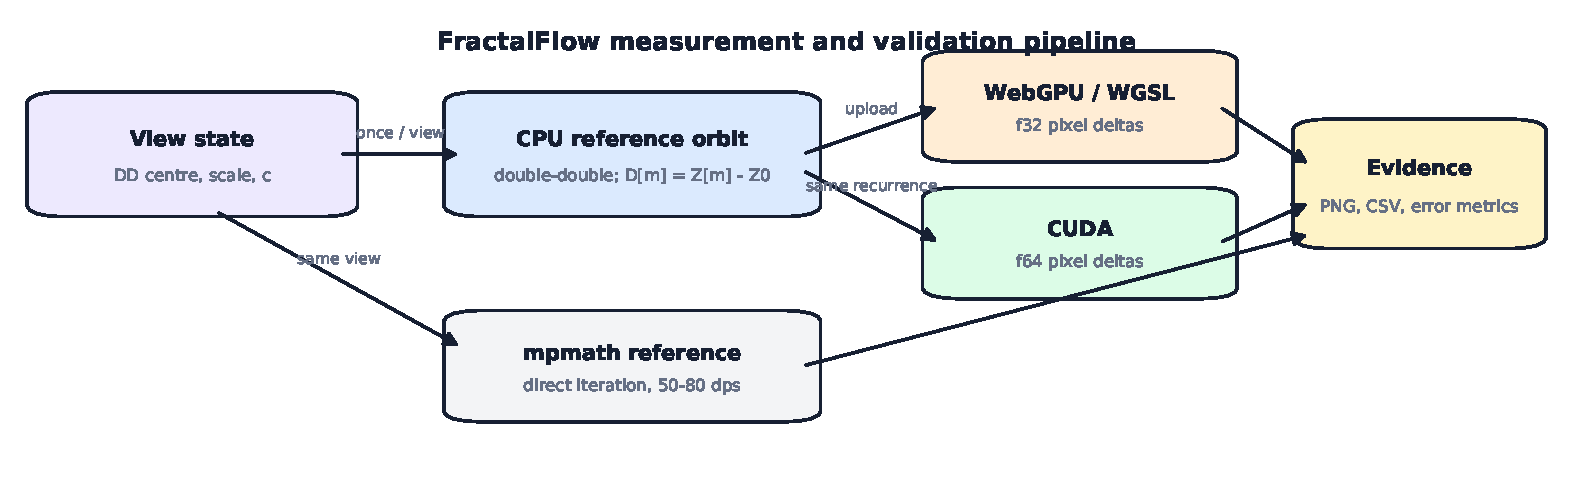
\includegraphics[width=\linewidth]{architecture.pdf}
  \caption{The precision-sensitive reference is computed once on the CPU.
  WebGPU and CUDA then evaluate the same per-pixel recurrence at different
  precisions. Direct arbitrary-precision iteration supplies an independent
  reference rather than reusing the implementation under test.}
  \label{fig:architecture}
\end{figure}

\section{Perturbation for a Julia map}

\subsection{Reference and delta recurrence}

Let \(Z_n\) be the reference orbit beginning at the view centre \(Z_0\):
\begin{equation}
  Z_{n+1}=Z_n^2+c.
  \label{eq:reference}
\end{equation}
A pixel begins at \(z_0=Z_0+\delta_0\), where \(\delta_0\) is its screen-space
offset after scale and aspect-ratio mapping. Writing \(z_n=Z_n+\delta_n\) and
substituting in Equation~\ref{eq:quadratic} gives
\begin{align}
  Z_{n+1}+\delta_{n+1}
    &= (Z_n+\delta_n)^2+c, \nonumber\\
  \delta_{n+1}
    &=2Z_n\delta_n+\delta_n^2.
  \label{eq:delta}
\end{align}
Unlike the corresponding Mandelbrot derivation, there is no \(\delta c\)
term: \(c\) is constant across a Julia image and the initial value varies per
pixel. Once \(Z_n\) is known, Equation~\ref{eq:delta} uses only ordinary complex
products and additions.

FractalFlow stores at most 4000 reference points. Each pixel maintains a
reference index \(m\), an iteration count and the complex delta. The escape
test uses \(z=Z_m+\delta\); escaped pixels terminate early, while interior
pixels stop at the iteration limit. Smooth coloring is applied only after the
escape decision and is kept identical between the measured renderers and the
Python reference.

\subsection{Rebasing}

A delta can cease to be small relative to its reference or the finite
reference orbit can run out. FractalFlow adapts the rebasing strategy credited
to Zhuoran and documented by Heiland-Allen \cite{heilandallen2022}. After a
delta advance, the implementation forms the pixel displacement from the
initial reference point,
\begin{equation}
  \delta^{(0)} = z-Z_0,
  \label{eq:rebase}
\end{equation}
and resets \(m\) to zero when
\(\lvert\delta^{(0)}\rvert < \lvert\delta\rvert\) or the next reference
sample is unavailable. The crucial expression is \(z-Z_0\), not \(z\).
These coincide only when \(Z_0=0\), which explains why an incorrect
Mandelbrot-style reset can remain hidden at the origin and fail in an
off-centre Julia view.

\section{Precision design}

\subsection{Double-double camera and orbit}

A double-double number represents a value as the unevaluated sum
\(x_{\mathrm{hi}}+x_{\mathrm{lo}}\) of two binary64 values. Error-free
transformations such as \textsc{TwoSum}, \textsc{QuickTwoSum} and Dekker's
split product recover the rounding residual of elementary operations
\cite{dekker1971,knuth1998,hida2000}. FractalFlow implements only addition,
subtraction and multiplication. The representation provides roughly 106
significand bits, or about 31 decimal digits, while retaining the binary64
exponent range.

The camera centre remains double-double through cursor-anchored zoom and pan.
The CPU also evaluates Equation~\ref{eq:reference} in double-double. The
browser does not emulate this arithmetic per pixel: doing so would replace a
small number of CPU operations with millions of compensated shader
operations. Instead, the reference is rounded once for GPU upload and the
pixel delta remains a native \texttt{f32}.

\subsection{Why the uploaded orbit is relative}

An early implementation uploaded absolute orbit samples
\(\mathrm{fl}_{32}(Z_m)\). This is sufficient for multiplying the small delta
by an approximate order-one \(Z_m\), but it is unsafe for Equation
\ref{eq:rebase}. Forming
\(\mathrm{fl}_{32}(Z_m)+\delta-Z_0\) subtracts nearby order-one values after
they have already been rounded to a grid whose spacing is approximately
\(10^{-7}\). At a view scale of \(10^{-10}\), many distinct pixel offsets
therefore collapse to zero or to the same grid point.

The current representation uploads
\begin{equation}
  D_m = \mathrm{fl}_{32}(Z_m-Z_0),
  \label{eq:relative}
\end{equation}
where the subtraction is performed in double-double on the CPU. The rebased
delta is then \(D_m+\delta\): both terms are small precisely when their sum
requires relative precision. The shader still reconstructs an approximate
\(Z_m\) for the recurrence as
\(\mathrm{fl}_{32}(Z_0)+D_m\), but the precision-critical subtraction is no
longer performed between two rounded order-one samples.

\begin{figure}[H]
  \centering
  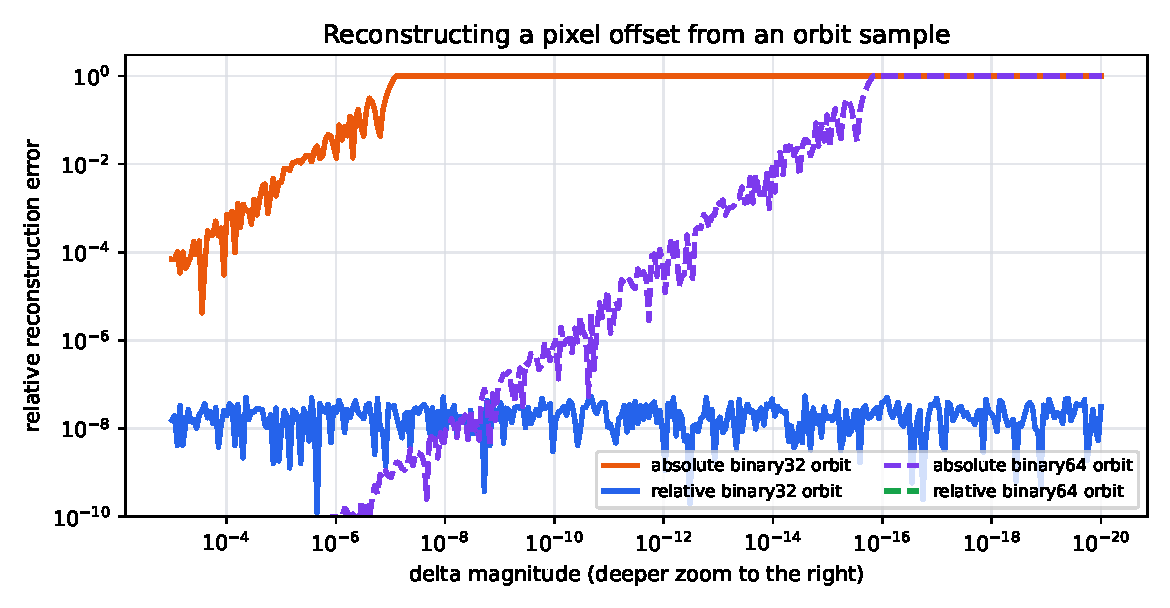
\includegraphics[width=0.88\linewidth]{relative_orbit_precision.pdf}
  \caption{Controlled binary32 experiment at the fixed point used in the
  validation suite. Encoding the absolute coordinate loses the delta once it
  falls below the local unit in the last place. Encoding the offset keeps an
  approximately constant relative error. This plot illustrates the
  quantization mechanism; it is not a renderer benchmark.}
  \label{fig:relative}
\end{figure}

\section{Three execution backends}

Figure~\ref{fig:architecture} summarizes the shared pipeline. The TypeScript
host owns the camera, computes the reference and selects a renderer through a
small common interface.

\paragraph{WebGPU.}
The primary browser backend uses a WGSL fragment shader and a storage buffer
for the relative reference orbit. WebGPU maps browser workloads to modern
native GPU APIs \cite{webgpu2026}; WGSL defines the portable shader language
and its host-shareable data layout \cite{wgsl2026}. Every fragment evaluates
Equation~\ref{eq:delta} in \texttt{f32}. A cached reference orbit is reused
until the view, Julia parameter or iteration limit changes.

\paragraph{CUDA.}
The native executable repeats the host-side double-double orbit calculation
and launches a CUDA kernel whose deltas are binary64. CUDA provides native
single- and double-precision arithmetic, but their throughput can differ
substantially by device class \cite{cuda2025}. The executable supports both PNG
rendering and a benchmark schedule identical to the browser harness.

\paragraph{WebGL2 fallback.}
The compatibility backend uses a double-single GLSL coordinate representation
and direct iteration. On the tested Windows ANGLE/D3D11 path, the compensated
arithmetic is not stable at the deepest scales; it is therefore neither used
as validation evidence nor included in the throughput chart. This exclusion
is important: the speed of a numerically wrong image is not a useful
performance result.

\clearpage
\thispagestyle{fancy}
\section{Correctness protocol}

\subsection{Independent reference}

The validation path performs direct iteration of Equation~\ref{eq:quadratic}
with \texttt{mpmath} at 50--80 decimal digits \cite{mpmath2026}. It contains no
reference orbit, perturbation or rebasing logic. Candidate and reference
renders share only the declared pixel mapping, escape radius, iteration limit
and color function. This independence is more useful than comparing the WGSL
and CUDA ports with each other because a shared algebraic error could make two
ports agree.

Four \(64\times64\) cases exercise distinct failure modes: an overview, an
off-centre boundary, a \(10^{-5}\) deep view and a \(10^{-10}\) view centred
on a repelling fixed point of \(z^2-0.8+0.156i\). The script records the mean
absolute RGB error, maximum channel error, percentage of identical pixels,
percentage whose three channels are all within four levels, and SHA-256 hashes
of both PNG files. A mean error of three levels is the release failure
threshold; the exact observations below are read from the archived CSV.

\begin{table}[H]
  \centering
  \small
  \caption{CUDA perturbation output versus direct \texttt{mpmath} rendering.
  Error units are 8-bit RGB levels, averaged over channels and pixels.}
  \label{tab:validation}
  \begin{tabular}{@{}lrrrrrrr@{}}
\toprule
Case & Scale & Iter.\ cap & Mean error & Max error & Pixels differing & By $>4$ & Flips \\
\midrule
Overview & $3$ & 300 & 0.000163 & 1 & 2 & 0 & 0 \\
Off-centre boundary & $3{\times}10^{-1}$ & 1100 & 0.169515 & 249 & 24 & 11 & 1 \\
Deep zoom & $10^{-5}$ & 700 & 0.000163 & 1 & 2 & 0 & 0 \\
Repelling fixed point & $10^{-10}$ & 400 & 0.000000 & 0 & 0 & 0 & 0 \\
Below binary64 & $10^{-16}$ & 700 & 0.000000 & 0 & 0 & 0 & 0 \\
Deepest validated & $10^{-20}$ & 1200 & 0.144206 & 251 & 20 & 9 & 2 \\
\bottomrule
\end{tabular}

\end{table}

\begin{figure}[H]
  \centering
  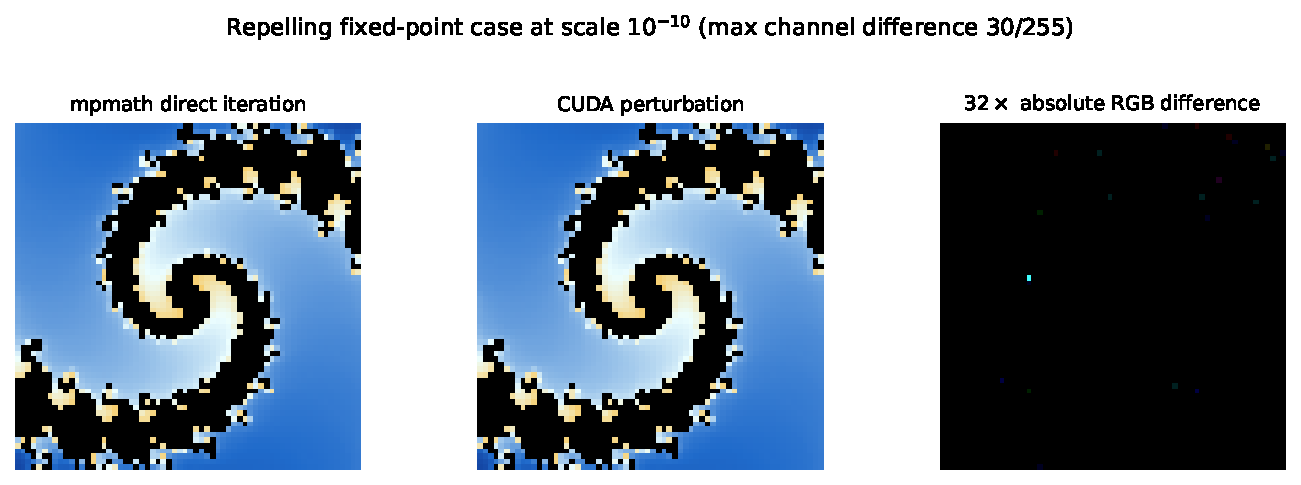
\includegraphics[width=0.92\linewidth]{validation_fixed_point.pdf}
  \caption{The most precision-sensitive fixed case. The third panel amplifies
  absolute channel differences by a factor of 32; the unamplified maximum is
  printed in the figure title by the generation script.}
  \label{fig:validation}
\end{figure}

The frozen pixel-level matrix covers CUDA, not WebGPU. The browser path shares
the tested TypeScript double-double and relative-orbit preparation, but advances
the delta in binary32 and is currently guarded only by unit tests plus the
benchmark luma readback. This is an explicit evidence gap: a future release
should export raw WebGPU pixels under automation and compare them with the same
\texttt{mpmath} reference. The current report therefore does not present the
CUDA image agreement as a universal proof for every backend.

\clearpage
\thispagestyle{fancy}
\section{Performance experiment}

\subsection{Method}

The benchmark uses 13 view scales \(3\times10^{-k}\), \(k=0,\ldots,12\), at
\(1920\times1080\). The iteration cap is
\(\min(300+800k,4000)\). For each depth, the browser reports the median of five
timed frames after three warm-up frames. Completion is synchronized with
\texttt{GPUQueue.onSubmittedWorkDone}; rendering targets an off-screen texture,
and a luma readback rejects silently black output. CUDA uses events around the
kernel. The reference orbit is prepared and cached before the timed region.

The reported iteration rate is
\begin{equation}
  R = \frac{W H I_{\max}}{t}.
  \label{eq:giter}
\end{equation}
This is an upper bound because escaped pixels terminate before \(I_{\max}\).
It remains useful for a controlled backend comparison because the schedule,
view, escape behavior and counting convention are shared. The NumPy baseline
\cite{numpy2020} times vectorized direct binary64 iteration for the shallow
anchor only and excludes coloring. The timed GPU kernels include their palette
evaluation and target writes; luma readback and file encoding remain outside
the timed region.

\begin{figure}[H]
  \centering
  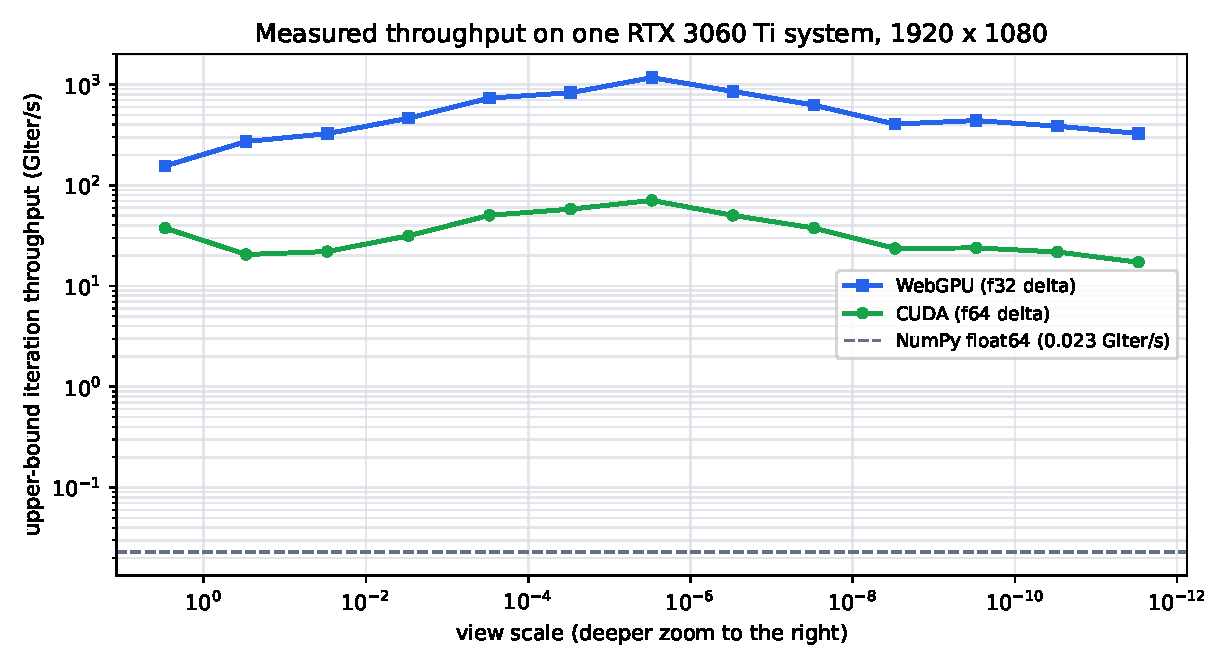
\includegraphics[width=0.92\linewidth]{benchmark_throughput.pdf}
  \caption{Frozen release measurements. The curves describe one software and
  hardware configuration, not WebGPU or CUDA in general. GIter/s uses the
  upper-bound convention in Equation~\ref{eq:giter}.}
  \label{fig:benchmark}
\end{figure}

\begin{table}[H]
  \centering
  \small
  \caption{Peak upper-bound GIter/s extracted from the archived CSV files,
  with Mpix/s from the same row. The CPU values refer to its single shallow
  anchor.}
  \label{tab:benchmark}
  \begin{tabular}{@{}lrrrr@{}}
\toprule
Backend & Peak GIter/s & Mpix/s & Frame (ms) & Scale \\
\midrule
WebGPU f32 & 1168.225 & 292.1 & 7.1 & $3{\times}10^{-6}$ \\
CUDA f64 & 70.774 & 17.7 & 117.2 & $3{\times}10^{-6}$ \\
NumPy f64 & 0.023 & 0.1 & 26476.6 & $3$ \\
\bottomrule
\end{tabular}

\end{table}
\thispagestyle{fancy}

\subsection{Interpretation}

The observed WebGPU peak is approximately 15.3 times the CUDA peak and roughly
51,000 times the NumPy GIter/s anchor. This does not imply that a browser is
intrinsically faster than native CUDA. The two GPU kernels execute different
precision choices: WebGPU uses binary32 deltas while CUDA uses binary64. On the
tested consumer Ampere device, the extra precision has a large throughput
cost. Perturbation makes the binary32 path viable by concentrating extended
precision in the single CPU reference orbit.

The curves also vary with depth because early escape, control-flow divergence
and the orbit structure change even when \(I_{\max}\) has reached its cap.
Consequently, a peak alone does not predict interactive frame time for an
arbitrary Julia parameter or viewport.

\clearpage
\thispagestyle{fancy}
\section{Reproducibility and limitations}

The release contains source code, lock files, benchmark CSVs, validation PNGs,
checksums and a figure-generation manifest. The essential commands are:

\begin{lstlisting}
npm ci
npm test
npm run build
nvcc -O3 cuda/julia.cu -o cuda/julia.exe
uv --cache-dir .uv-cache run python scripts/validate_release.py
cuda/julia.exe --bench --w 1920 --h 1080 \
  --out paper/data/benchmark/cuda_bench.csv
uv --cache-dir .uv-cache run python paper/generate_figures.py
latexmk -cd -norc -pdf paper/main.tex
\end{lstlisting}

The WebGPU CSV is generated at \texttt{/?bench=webgpu}; the page also emits a
machine-readable console record. The report PDF is rebuilt in CI with TeX Live
2026. The software release is licensed under Apache-2.0, while this report and
its original figures are CC BY 4.0.

The evidence has five main limitations. First, performance is measured on one
RTX 3060 Ti system and one browser/driver stack. Second, RGB comparison can
hide compensating differences in raw iteration state, although the identical
color mapping and fixed cases make large errors visible. Third, one reference
orbit and the current rebasing rule are not a proof of correct rendering for
every Julia parameter. Fourth, the WebGL2 fallback is a compatibility path,
not a validated deep-zoom backend on the tested ANGLE configuration. Finally,
double-double limits the current camera to roughly 31 decimal digits; it is
not an arbitrary-depth representation.

\section{Conclusion}

FractalFlow demonstrates a practical division of numerical labor: compute one
reference orbit with extended precision, then spend the GPU budget on cheap
per-pixel deltas. The portable recurrence is short; the difficult part is
preserving the meaning of a small delta at every representation boundary.
Storing \(Z_m-Z_0\) rather than \(Z_m\) makes the rebasing path scale with the
view and removes an order-one binary32 quantization failure. Independent
arbitrary-precision renders and frozen benchmark inputs turn that observation
into a checkable software result. Future work includes raw iteration-state
validation, additional devices and browsers, series approximation, progressive
tiling and a higher-precision camera beyond \(10^{-28}\)-scale views.

\thispagestyle{fancy}
\begingroup
\scriptsize
\bibliographystyle{unsrt}
\bibliography{references}
\endgroup

\medskip
\noindent\footnotesize
\textbf{Licensing.} Copyright 2026 Timofei Amosov. This report is licensed
under CC BY 4.0. FractalFlow version 1.1.0 is licensed under Apache-2.0.

\end{document}
